% ----------------------------------------------------------------------
%  Základní nastavení dokumentu - musí být na začátku každého tex
%  (pořadí příkazů v této části je důležité!)
% ----------------------------------------------------------------------

%  Typ dokumentu - článek, prezentace aj.
% Standardní základ
%\documentclass[a4paper,10pt]{article} 
%\usepackage[letterpaper]{geometry}
%\geometry{verbose,tmargin=1.5cm,bmargin=2cm,lmargin=2cm,rmargin=2cm}

% Alternativní verze - vhodnější formát papíru (větší hustota textu)
\documentclass[10pt]{scrartcl}
\KOMAoptions{DIV=20} % formát papíru a odsazení od jeho okrajů

%  Kódování výstupu - aby šlo z pdf kopírovat včetně háčků a čárek
\usepackage[T1]{fontenc} 

%  Kódování vstupu - v kódu lze použít háčky a čárky
\usepackage[utf8]{inputenc} 

%  Základní typografická pravidla češtiny/slovenštiny
\usepackage[czech]{babel} 
%\usepackage[slovak]{babel}
% použijte jen jeden z příkazů


%  Lépe vypadající písmo pro T1 kódování
\usepackage{lmodern} 
% je možno zakomentovat, nepoužívá-li se T1 kódování




%  Formátování stránek, empty = odstraní číslování
% \pagestyle{empty}

%  Řádkování
\linespread{1.1}

% vynuceni pevne pozice obrazku
\usepackage{float}


% ----------------------------------------------------------------------
%  Doplňující balíčky
% ----------------------------------------------------------------------

%  Po desetinné čárce v matematickém módu se nevytvoří mezera
\usepackage{icomma} 

%  Umožňuje pracovat s grafikou
\usepackage[rightcaption]{sidecap}
\usepackage{graphicx}
\usepackage{subfig}
\usepackage{subcaption}

%  Umožňuje použít dva obrázky vedle sebe
\usepackage{subcaption}

%  Pro vkládání obrázků ve formátu eps (např. z gnuplot)
\usepackage{epstopdf} 

%  Automaticky odsadí i první paragraf v každé sekci
\usepackage{indentfirst}

%  Umožňuje rozdělovat obsah na více sloupců
\usepackage{multicol}
\usepackage{booktabs}
\usepackage{pgffor}

%  Umožňuje používat hypertextové odkazy, nastavuje jejich vlastnosti
\usepackage[unicode]{hyperref}


% ----------------------------------------------------------------------
%  Matematika
% ----------------------------------------------------------------------

%  Lepší zobrazování matematiky (rozšíření sum o \limits atd.)
\everymath{\displaystyle}

%  Široké spektrum příkazů pro matematiku
% (Umožní např. psát přes \mathbb{N/R/Q/..} množiny čísel)
\usepackage{amsmath,amssymb}

%  Velikost fontu matematických výrazů v dokumentu lze pro danou
% základního fontu dokumentu upravit pomocí:
% \DeclareMathSizes{X}{Y}{Z}{U} kde:
% X je velikost fontu v dokumentu, pro kterou se matematika upraví
% Y je standartní velikost fontu matematiky
% Z je velikost fontu zmenšených (vnořených výrazů)
% U je velikost fontu ještě více zmenšených (vnořených výrazů).
\DeclareMathSizes{10}{10}{8}{7}

%  Široké spektrum příkazů pro fyziku
\usepackage{physics}

%  Psaní SI jednotek
\usepackage{siunitx}

%  Nám bližší zápis písmene epsilon
\AtBeginDocument{%
%\let\phi\varphi
\let\epsilon\varepsilon
}


% ----------------------------------------------------------------------
%  Pro češtinu/slovenštinu
% ----------------------------------------------------------------------

%  Lokalizace některých názvů do češtiny/slovenštiny
\addto\captionsczech{\renewcommand{\figurename}{Obr.}}
\addto\captionsczech{\renewcommand{\tablename}{Tab.}}
%\addto\captionsczech{\renewcommand{\refname}{Reference}}

\addto\captionsslovak{\renewcommand{\figurename}{Obr.}}
\addto\captionsslovak{\renewcommand{\tablename}{Tab.}}
%\addto\captionsslovak{\renewcommand{\refname}{Reference}}

% Odkomentujte následující příkaz, máte-li stažený balíček encxvlna 
% (nutno stáhnout manuálně)
%\usepackage{encxvlna} %vloží nezlomitelné mezery k jednopísmenným



% ----------------------------------------------------------------------
%  Soubor s makry
% ----------------------------------------------------------------------
% ----------------------------------------------------------------------
%  Identifikace protokolu (příkazy lze použít v celém dokumentu)
% ----------------------------------------------------------------------

%  Nastaví autora, název, datum, skupinu měření apod. 
\newcommand{\Institute}{FJFI~ČVUT~v~Praze}
%\newcommand{\Subject}{Základy fyzikálních měření}
\newcommand{\Subject}{Základní praktika z laserové techniky}  %odkomentujte dle potřeby

%  Máte-li více spoluměřících než jednoho, vložte jen jejich příjmení
\newcommand{\Author}{B -- Hrnečková, Ray}
\newcommand{\Coauthor}{Jméno kolegy} 
\newcommand{\Group}{Pátek 8:00} %den, kdy chodíte na praktika, nikoli obor
\newcommand{\Circle}{2} %číslo skupiny v rámci praktika, nikoli kruh

%  Tato část bude v každém protokolu jiná, nezapomeňte upravit!
\newcommand{\Title}{Pevnolátkový Nd:YAG laser v režimu volné generace a v režimu Q-spínání,
zesilování laserového záření a generace druhé harmonické}
\newcommand{\Labdate}{19. 3. 2025} %datum měření, nikoli datum odevzdání
\newcommand{\Worktime}{5 h} %jak dlouho vám trvalo vypracování protokolu




% ----------------------------------------------------------------------
%  Vlastní příkazy
% ----------------------------------------------------------------------


%  Matematika
\newcommand{\ee}{\mathrm{e}} %eulerovo číslo
\newcommand{\ii}{\mathrm{i}} %imaginární jednotka

% Jednotky
\renewcommand{\unit}[1]{\,\mathrm{#1}} %jednotky zadávejte pomocí tohoto příkazu
\renewcommand{\deg}{\ensuremath{\mathring{\;}}} %symbol stupně
\newcommand{\celsius}{\ensuremath{\deg\mathrm{C}}} %stupně celsia

%(hodnota plus mínus chyba) jednotka
\newcommand{\hodn}[3]{(#1 \pm #2)\unit{#3}} 

%veličina [jednotka] do hlavičky tabulky
\newcommand{\tabh}[2]{\ensuremath{#1\,[\mathrm{#2}]}} 

%  nachází se ve složce /tex/



% ----------------------------------------------------------------------
%  Nastavení odkazů a výsledného pdf
% ----------------------------------------------------------------------
\hypersetup{
colorlinks=true, 
citecolor=blue, 
filecolor=blue, 
linkcolor=blue,
urlcolor=blue, 
pdftitle={\Title},    % title
pdfauthor={\Author},     % author
pdfsubject={Protokol},   % subject of the document
pdfcreator={\Author},   % creator of the document
%     pdfproducer={Producer}, % producer of the document
%     pdfkeywords={keywords}, % list of keywords
pdfnewwindow=true,      % links in new window
}

% ----------------------------------------------------------------------
%  Začátek dokumentu - formátování na výstup
% ----------------------------------------------------------------------
\begin{document}

% Interní proměnné, možno zobrazovat u prezentací, používají se při
% generování pomocí \titlepage apod.
\author{\Author}
\title{\Title}
\date{\Labdate}


% ----------------------------------------------------------------------
%  Hlavička dokumentu
% ----------------------------------------------------------------------

\setlength{\parindent}{0cm}
\begin{multicols}{2}
\textsf{\textbf{\Subject \hspace{7.75cm} \Institute}\\
%\large  \Title \\[0.5cm]
\textbf{\large{\Title}}}

\begin{tabular}{rlrl}
	 \textsf{Skupina:} & \textbf{\textsf\Author}    &   \textsf{Měřeno:} & \textbf{\textsf{\Labdate}}    
\end{tabular}

\begin{flushright}


\includegraphics[scale=0.2]{img/fjfi.pdf}
\hspace{0.4cm}

\includegraphics[scale=0.2]{img/cvut.pdf}

\begin{flushleft}
%\hspace{3.64cm} \textsf{Náročnost/Zábavnost: 1/5} \\
\end{flushleft} 
\textsf{Klasifikace:} \hspace{3.2cm} 

\end{flushright}
\end{multicols}

\hrule

% ----------------------------------------------------------------------
%  Tělo dokumentu
% ----------------------------------------------------------------------

\setlength{\parindent}{0.5cm}

% ----------------------------------------------------------------------
%  Protokol

\pagenumbering{arabic}  % číslování stránek čísly
% ----------------------------------------------------------------------
%  Před psaním se důkladně seznamte s Pravidly pro vypracování protokolu!
% ----------------------------------------------------------------------

% ----------------------------------------------------------------------
%  Pracovní úkoly - opište přímo ze zadání
% ----------------------------------------------------------------------
%\section{Pracovní úkoly}

%\begin{enumerate}
%\item ...

%\end{enumerate}

% ----------------------------------------------------------------------
%  Použité pomůcky
% ----------------------------------------------------------------------

%\newpage


%\begin{figure}[H]
%	\centering
%	\includegraphics[scale = 0.5]{img/schema_regulovane_soustavy.png} 
%	\caption{Schéma regulované soustavy.} 
%	\label{fig:schema_reg}
%\end{figure}	

%\begin{figure}[H] 
%	\centering
%	\includegraphics[scale = 0.7]{img/schema_PID_regulatoru.png} 
%	\caption{Schéma PID regulátoru.} 
%	\label{fig:schema_PID}
%\end{figure}		
		

% ----------------------------------------------------------------------
%  Teoretický úvod - vlastními slovy stručne popište fyzikální podstatu měření a uveďte základní vztahy použité ve vypracování
% ----------------------------------------------------------------------
%\section{Teoretický úvod}	

% ----------------------------------------------------------------------
%  Postup měření - vlastními slovy popište postup měření tak, aby bylo vaše měření reprodukovatelné 
% ----------------------------------------------------------------------
%\section{Postup měření}
			
% ----------------------------------------------------------------------
%  Naměřené hodnoty a samotné vypracování úkolu
% ----------------------------------------------------------------------	
			
\section{Vypracování}
\subsection{Charakteristika laseru v režimu volné generace}
Závislosti výstupní energie $E$ a účinnosti $\eta$ na budící energii $E_\mathrm{b}$ pro zrcadla M337, M327 a křemenné sklo jsou uvedeny v Tab.~\ref{tab:ucinnost_zrcadla} a v grafech na Obr.~\ref{fig:ucinnost_M337},~\ref{fig:ucinnost_kremenne_sklo},~\ref{fig:ucinnost_M327}.

Závislost délky impulsu $\tau_\mathrm{FR}$, a středního výkonu $P_\mathrm{str}$ na budící energii $E_\mathrm{b}$ pro pro optimální zrcadlo (M327) je uvedena v Tab.~\ref{tab:optimalni_zrcadlo} a vykreslena na Obr.~\ref{fig:optimalni_zrcadlo}.\\
Hustota energie při maximální energii $\rho_\mathrm{max}=8,73\unit{J\cdot cm^{-2}}$ \\
Obrázky časových průběhů záření jsou na Obr.~\ref{fig:cas_1},~\ref{fig:cas_2}~a~\ref{fig:cas_3}.

\begin{table}[!hbt]
\centering
	\begin{tabular}{|c|c|c||c|c|c||c|c|c|}
		\hline
		\multicolumn{3}{|c||}{M337}					&	\multicolumn{3}{c||}{křemenné sklo}					&	\multicolumn{3}{c|}{M327}					\\ \hline
$\tabh{E_\mathrm{b}}{J}$	&	\tabh{E}{J}	&	\tabh{\eta}{\%}	&	$\tabh{E_\mathrm{b}}{J}$	&	\tabh{E}{J}	&	\tabh{\eta}{\%}	&	$\tabh{E_\mathrm{b}}{J}$	&	\tabh{E}{J}	&	\tabh{\eta}{\%}	\\ \hline \hline
13,62	&	0,00	&	0,00	&	15,21	&	0,00	&	0,00	&	13,76	&	0,00	&	0,00	\\ \hline
14,14	&	0,02	&	0,16	&	16,89	&	0,02	&	0,11	&	14,14	&	0,02	&	0,15	\\ \hline
15,21	&	0,04	&	0,29	&	19,27	&	0,08	&	0,40	&	15,21	&	0,07	&	0,45	\\ \hline
16,89	&	0,07	&	0,39	&	22,37	&	0,15	&	0,68	&	16,89	&	0,13	&	0,74	\\ \hline
19,27	&	0,10	&	0,50	&	26,52	&	0,24	&	0,89	&	19,27	&	0,19	&	1,01	\\ \hline
22,37	&	0,14	&	0,60	&	31,70	&	0,35	&	1,10	&	22,37	&	0,27	&	1,21	\\ \hline
26,52	&	0,19	&	0,71	&	34,22	&	0,39	&	1,14	&	26,52	&	0,34	&	1,30	\\ \hline
31,70	&	0,25	&	0,78	&	38,32	&	0,47	&	1,24	&	31,70	&	0,45	&	1,41	\\ \hline
38,32	&	0,33	&	0,87	&	42,90	&	0,56	&	1,30	&	38,32	&	0,58	&	1,51	\\ \hline
46,38	&	0,40	&	0,85	&	48,16	&	0,66	&	1,37	&	46,38	&	0,72	&	1,55	\\ \hline
56,25	&	0,51	&	0,90	&	56,25	&	0,81	&	1,44	&	56,25	&	0,89	&	1,58	\\ \hline

	\end{tabular}
	\caption{Závislosti výstupní energie $E$ a účinnosti $\eta$ na budící energii $E_\mathrm{b}$ pro zrcadla M337, M327 a křemenné sklo.}
	\label{tab:ucinnost_zrcadla}
\end{table}

\begin{figure}[H] 
	\centering
	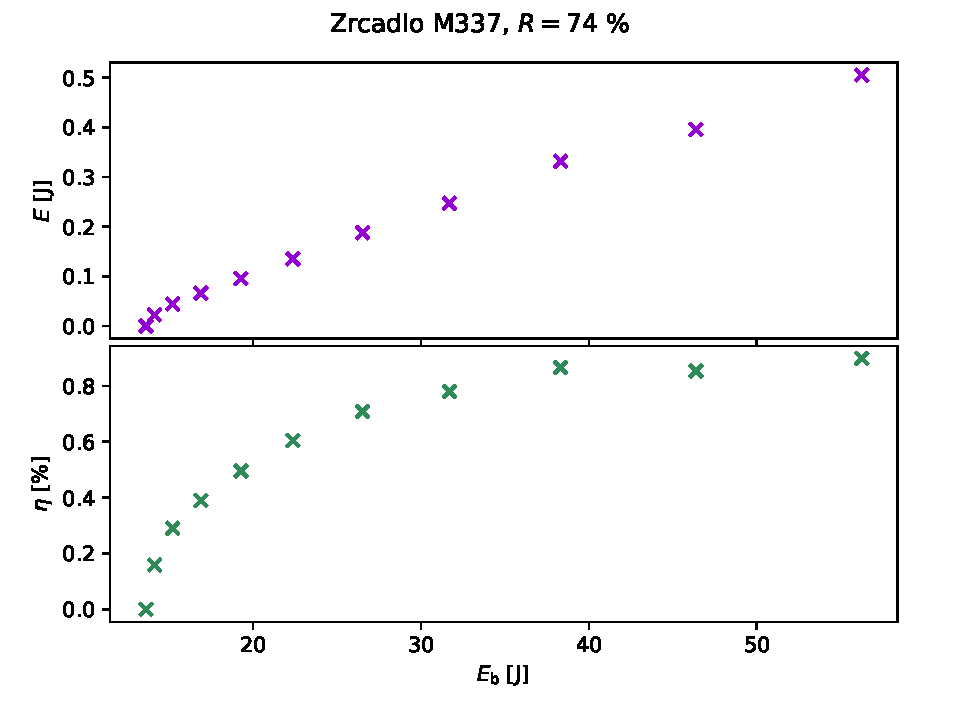
\includegraphics[scale = 0.7]{img/zrcadlo_M337.pdf} 
	\caption{Závislost výstupní energie $E$ a účinnosti $\eta$ na budící energii $E_\mathrm{b}$ pro zrcadlo M337.} 
	\label{fig:ucinnost_M337}
\end{figure}


\begin{figure}[H] 
	\centering
	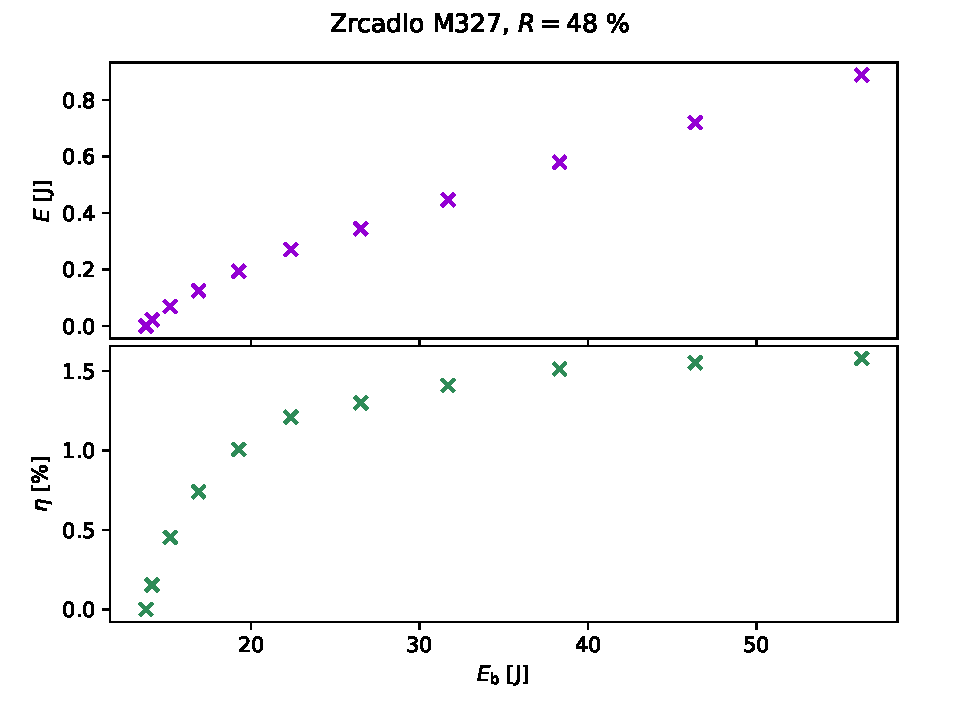
\includegraphics[scale = 0.7]{img/zrcadlo_M327.pdf} 
	\caption{Závislost výstupní energie $E$ a účinnosti $\eta$ na budící energii $E_\mathrm{b}$ pro zrcadlo M327.} 
	\label{fig:ucinnost_M327}
\end{figure}


\begin{figure}[H] 
	\centering
	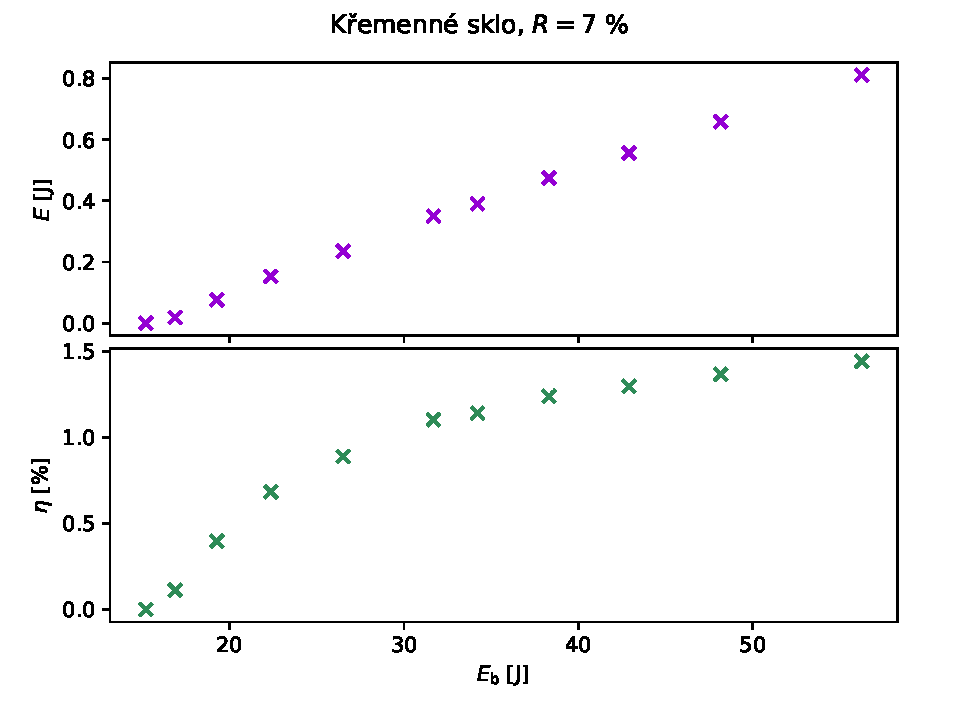
\includegraphics[scale = 0.7]{img/zrcadlo_kremenne_sklo.pdf} 
	\caption{Závislost výstupní energie $E$ a účinnosti $\eta$ na budící energii $E_\mathrm{b}$ pro zrcadlo z křemenného skla.} 
	\label{fig:ucinnost_kremenne_sklo}
\end{figure}


\begin{table}[!hbt]
\centering
	\begin{tabular}{|c||c|c|}
		\hline
$\tabh{E_\mathrm{b}}{J}$ & \tabh{\tau}{\mu s} & $\tabh{P_\mathrm{str}}{kW}$ \\ \hline \hline
13,76 & 63 & 0 \\ \hline
31,70 & 308 & 1,450 \\ \hline
56,25 & 83 & 10,674 \\ \hline
	\end{tabular}
	\caption{Závislost délky impulsu $\tau_\mathrm{FR}$, a středního výkonu $P_\mathrm{str}$ na budící energii $E_\mathrm{b}$ pro zrcadlo M327.}
	\label{tab:optimalni_zrcadlo}
\end{table}

\begin{figure}[H] 
	\centering
	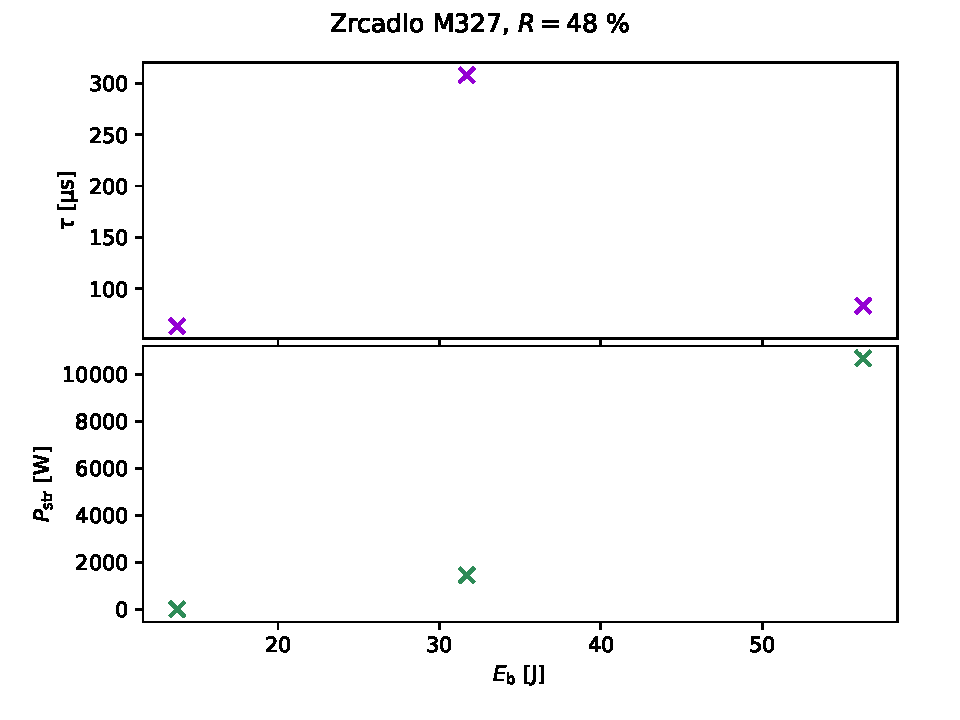
\includegraphics[scale = 0.7]{img/optimalni_zrcadlo.pdf} 
	\caption{Závislost délky impulsu $\tau_\mathrm{FR}$, a středního výkonu $P_\mathrm{str}$ na budící energii $E_\mathrm{b}$ pro zrcadlo M327.} 
	\label{fig:optimalni_zrcadlo}
\end{figure}

\begin{figure}[H] 
	\centering
	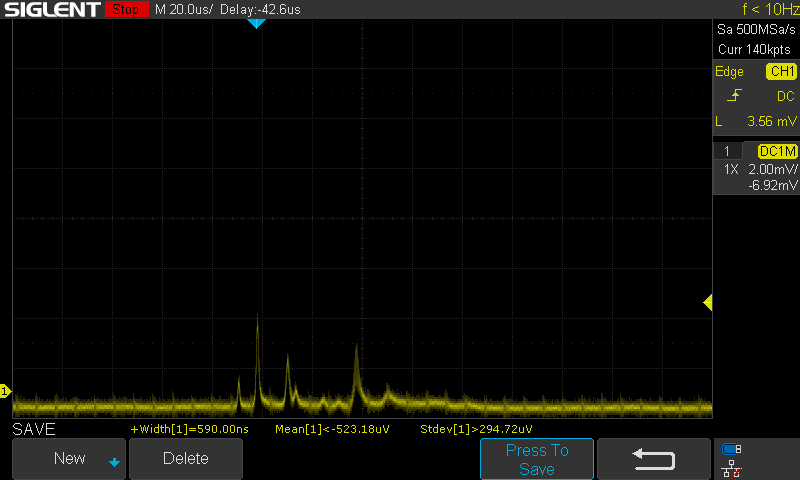
\includegraphics[scale = 0.5]{img/SDS00002.png} 
	\caption{Časový průbeh impulsu pro $E_\mathrm{b}$=13,76 J} 
	\label{fig:cas_1}
\end{figure}

\begin{figure}[H] 
	\centering
	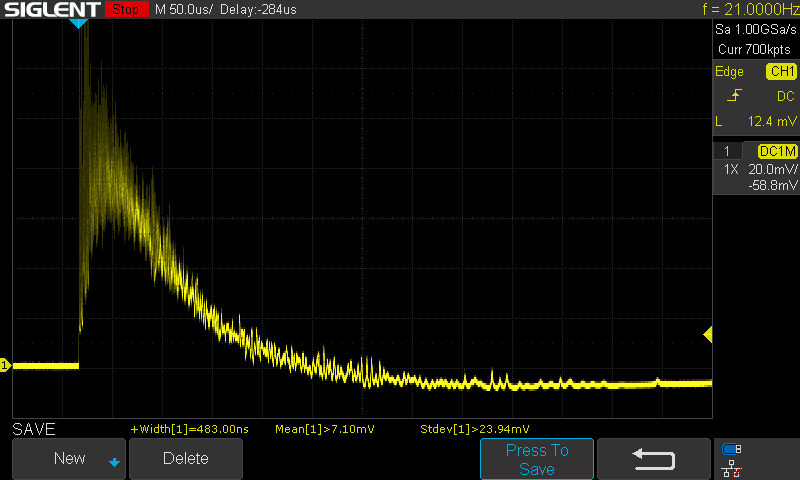
\includegraphics[scale = 0.5]{img/SDS00004.png} 
	\caption{Časový průbeh impulsu pro $E_\mathrm{b}$=31,70 J} 
	\label{fig:cas_2}
\end{figure}

\begin{figure}[H] 
	\centering
	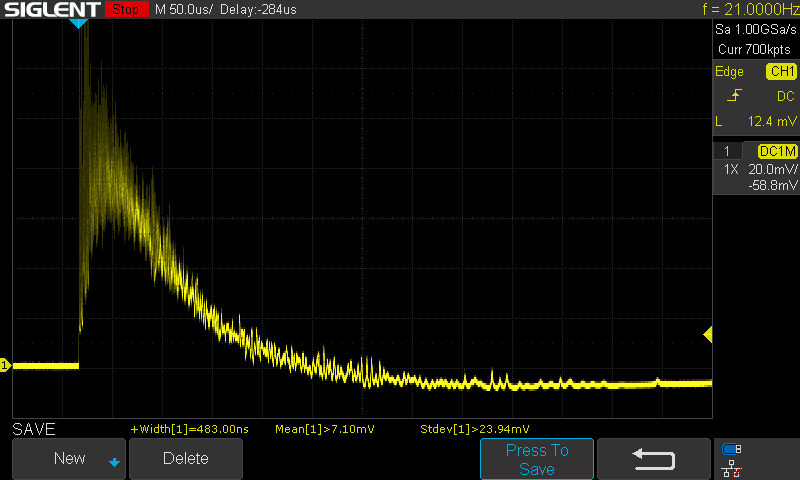
\includegraphics[scale = 0.5]{img/SDS00004.png} 
	\caption{Časový průbeh impulsu pro $E_\mathrm{b}$=65,25 J} 
	\label{fig:cas_3}
\end{figure}


\subsection{Zesilování impulsů}
Závislost zesílení impulsu $G$ na budící energii $E_\mathrm{b}$ laserového oscilátoru pro optimální zrcadlo (M327) je na Obr.\ref{fig:zasileni}.
\begin{figure}[H] 
	\centering
	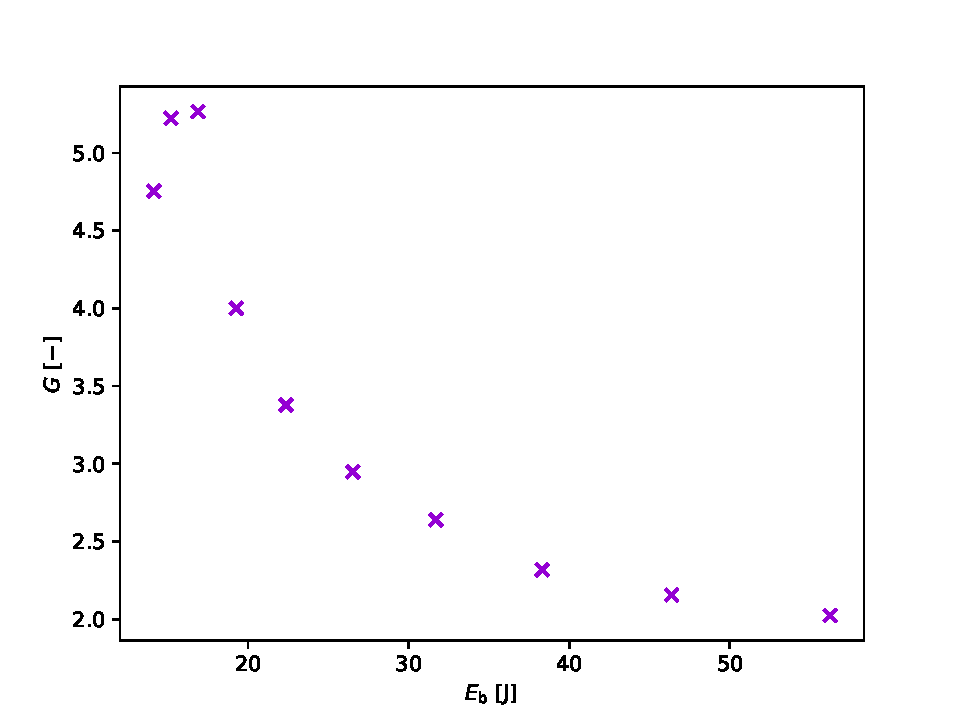
\includegraphics[scale = 0.7]{img/zesileni.pdf} 
	\caption{Závislost zesílení impulsu $G$ na budící energii $E_\mathrm{b}$ laserového oscilátoru pro zrcadlo M327.} 
	\label{fig:zasileni}
\end{figure}

\subsection{Q-spínaný režim}
Výsledky měření délky $\tau$, energie $E$, špičkového výkonu $P_\mathrm{peak}$ a plošné hustoty energie $\rho$ Q-spínaných impulsů jsou v Tab.~\ref{tab:q_spinani}. \\
Hustota energie v Q-spínaném režimu je oproti režimu volné generace přibližně $100\times$ vyšší.
Záznam časového vývoje z osciloskopu

\begin{table}[!hbt]
\centering
	\begin{tabular}{|c|c|c|c|c|}
		\hline
	&	\tabh{\tau}{ns}	&	\tabh{E}{mJ}	&	$\tabh{P_\mathrm{peak}}{kW}$	&	\tabh{\rho}{J\cdot cm^{-2}}	\\ \hline	\hline
	&	25	&	51	&	2075	&	773	\\ \hline	
	&	24	&	51	&	2145	&	773	\\ \hline	
	&	27	&	54	&	2042	&	819	\\ \hline	
	&	30	&	65	&	2154	&	981	\\ \hline	
	&	26	&	52	&	2000	&	784	\\ \hline	
	&	22	&	48	&	2245	&	734	\\ \hline	
	&	28	&	67	&	2362	&	1008	\\ \hline	
	&	26	&	45	&	1761	&	680	\\ \hline	
	&	25	&	66	&	2612	&	1005	\\ \hline	
	&	25	&	52	&	2048	&	784	\\ \hline	\hline
Průměr	&	26	&	55	&	2144	&	834	\\ \hline	
Odchylka	&	2	&	7	&	216	&	113	\\ \hline	


	\end{tabular}
	\caption{Výsledky měření délky $\tau$, energie $E$, špičkového výkonu $P_\mathrm{peak}$ a plošné hustoty energie $\rho$ Q-spínaných impulsů.}
	\label{tab:q_spinani}
\end{table}


\begin{figure}[H] 
	\centering
	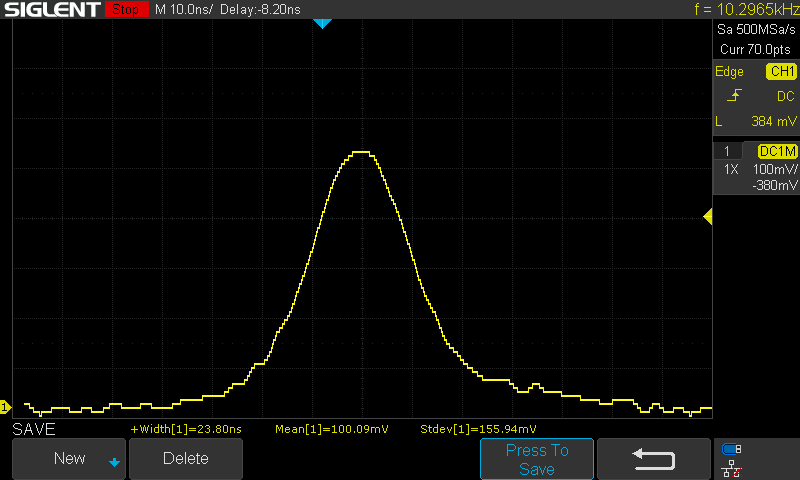
\includegraphics[scale = 0.5]{img/SDS00008.png} 
	\caption{Záznam časového vývoje z osciloskopu pro Q-spínaný puls.}
	\label{fig:cas_3}
\end{figure}
% ----------------------------------------------------------------------
%  Diskuse - obsahuje komentář k jednotlivým výsledkům, porovnání s očekáváním/tabulkovými hodnotami, zdroje především systematických chyb měření, návrh na zlepšení výsledků,...
% ----------------------------------------------------------------------			
%\section{Diskuse}			

% ----------------------------------------------------------------------
%  Závěr - stručně a jasně shrnout splněné cíle měření, úkoly a výsledky měření
% ----------------------------------------------------------------------
			
%\section{Závěr}




% ----------------------------------------------------------------------

% ----------------------------------------------------------------------
%  Literatura

%\section{Použitá literatura}		
%\begingroup
%\renewcommand{\section}[2]{}
%% ----------------------------------------------------------------------
%  Reference
% ----------------------------------------------------------------------

% sem doplňujte použité zdroje


%\endgroup
% ----------------------------------------------------------------------


% ----------------------------------------------------------------------
%  Příloha

%\clearpage 
%\pagenumbering{roman}  % číslování stránek písmeny

%\setcounter{equation}{0}
%\setcounter{section}{0}
%\numberwithin{equation}{section} % případné rovnice budou číslované pod číslem kapitoly

%\part*{\LARGE{Příloha}}

%% ----------------------------------------------------------------------
%  Příloha
% ----------------------------------------------------------------------

% Pokud chcete odsadit přílohu na novou stránku, odkomentujte toto
%\clearpage


% ----------------------------------------------------------------------

%\clearpage
				
%\clearpage


\end{document}

% ----------------------------------------------------------------------
%  Konec dokumentu
% ----------------------------------------------------------------------
